%!TEX program = xelatex 
\documentclass{standalone}
\usepackage{pgfplots}
\usepackage{units}
\pgfplotsset{compat=1.8}% <-- moves axis labels near ticklabels
                        % (respects tick label widths)
\usepackage{tikz,tikz-3dplot}
\usetikzlibrary{arrows, positioning, calc, intersections, decorations.markings}

\begin{document}

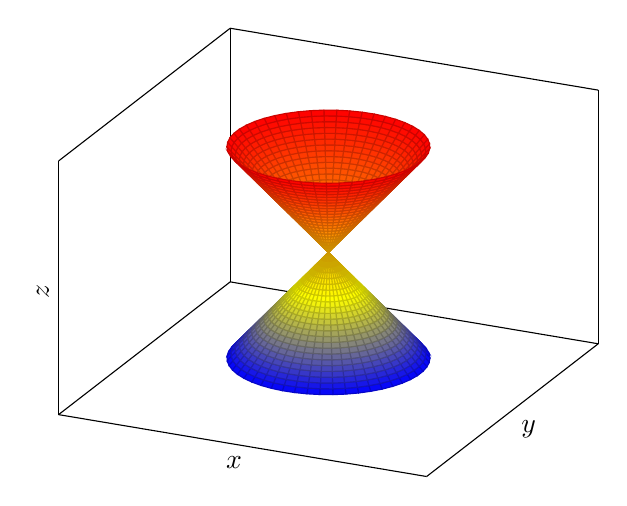
\begin{tikzpicture}
    % \begin{axis}[%
    %     width=25cm,
    %     height=25cm,
    %     ticks=none,
    %     xmin=-7, xmax=13, ymin=-2, ymax=2, zmin=-4, zmax=4,
    %     axis lines = center,
    %     xlabel=$x$,ylabel=$y$,zlabel=$z$,
    %     view={120}{30},
    %     domain = 0:5,
    %     y domain = 0:2*pi,
    % ]
    % \addplot3[%
    %     opacity = 0.5,
    %     surf,
    %     z buffer = sort,
    %     samples = 50,
    % ]
    % ({x*cos(deg(y))}, {x*sin(deg(y))}, {x});
    % \addplot3[%
    %     opacity = 0.5,
    %     surf,
    %     z buffer = sort,
    %     samples = 50,
    % ]
    % ({x*cos(deg(y))}, {x*sin(deg(y))}, {-x});
    % \end{axis}

    \begin{axis}[
domain=-5:5,
y domain=0:2*pi,
xmin=-10,
xmax=10,
ymin=-10,
ymax=10,
ticks=none,
xlabel=$x$,
ylabel=$y$,
zlabel=$z$,
samples=50]
\addplot3 [surf,z buffer=sort] 
({x*cos(deg(y))},
{x*sin(deg(y))},
{x} );
\end{axis}
\end{tikzpicture}
\end{document}